\documentclass[12pt,a4paper]{report}
\usepackage[utf8]{inputenc}
\usepackage{amsmath}
\usepackage{amsfonts}
\usepackage{amsthm}
\usepackage{mathtools}
\usepackage{amssymb}
\usepackage{natbib}
\usepackage{polski}
\usepackage{xcolor}
\usepackage{url}
\usepackage{algorithm}
\usepackage{algorithmicx}
\usepackage{algpseudocode}

\usepackage{hyperref}
\usepackage[polish, chapter]{dyschemist}
\usepackage[left=2cm,right=2cm,top=2cm,bottom=2cm]{geometry}


\newcommand{\vr}[1]{\mathbf{#1}}
\newcommand{\mx}[1]{{#1}}
\newcommand{\sign}{\operatorname{sign}}
\newcommand{\proj}[2]{\frac{\scalar{#2}{#1}}{\scalar{#1}{#1}}}


\usepackage{Sweave}
\begin{document}
\Sconcordance{concordance:licencjat.tex:licencjat.Rnw:%
1 26 1 1 0 912 1 1 10 12 0 1 2 2 1 1 19 21 0 1 2 6 1 1 14 16 0 1 2 2 1 %
1 16 18 0 1 2 17 1 1 2 1 0 1 1 3 0 1 2 2 1 1 2 4 0 1 2 2 1 1 2 4 0 1 2 %
2 1 1 2 4 0 1 2 11 1 1 2 1 0 3 1 6 0 1 2 2 1 1 2 1 0 3 1 6 0 1 2 2 1 1 %
2 1 0 3 1 6 0 1 2 9 1 1 2 4 0 1 2 2 1 1 2 4 0 1 2 2 1 1 2 4 0 1 2 2 1 1 %
2 4 0 1 2 4 1 1 2 1 0 3 1 6 0 1 2 1 1 1 2 1 0 3 1 6 0 1 2 1 1 1 2 1 0 3 %
1 6 0 1 2 9 1 1 2 4 0 1 2 5 1 1 2 4 0 1 2 2 1 1 2 4 0 1 2 2 1 1 2 4 0 1 %
2 3 1 1 2 1 0 3 1 6 0 1 2 2 1 1 2 1 0 3 1 6 0 1 2 1 1 1 2 1 0 3 1 6 0 1 %
2 8 1 1 2 1 0 3 1 3 0 1 2 1 3 1 0 2 1 1 2 5 0 1 2 25 1}



\begin{titlepage}
\begin{flushleft}
\end{flushleft}
\begin{center}
\textsc{{\huge Politechnika Łódzka}}
\end{center}
\bigskip
\bigskip
\begin{center}
\textsc{{\Large Wydział Fizyki Technicznej, Informatyki i Matematyki Stosowanej}}
\end{center}
\bigskip
\bigskip
%\begin{center}
\begin{Large}
Kierunek: Matematyka\\   
Specjalność: Matematyczne Metody Analizy Danych Biznesowych %TU WPISZ SPECJALNOŚĆ% 

\end{Large}
%\end{center}
\bigskip
\bigskip
\bigskip
\bigskip
\noindent\hrulefill
\begin{center}
\textsc{\textbf{{\Large Algorytmy dekompozycji QR %TU WPISZ TYTUŁ PRACY%
\\}}}
\end{center}
\bigskip
\bigskip
\begin{flushright}
{\large 
Anna Szczepaniak %TU WPISZ SWOJE IMIĘ I NAZWISKO%
\\
Nr albumu: 
210094 %TU WPISZ SWÓJ NUMER ALBUMU%
\\}
\end{flushright}
\noindent\hrulefill
\bigskip
\bigskip
\bigskip
\bigskip
\begin{center}
{\large Praca licencjacka\\ %TU WPISZ RODZAJ PRACY DYPLOMOWEJ: magisterska/licencjacka%
napisana w Instytucie Matematyki Politechniki Łódzkiej\\ 
\bigskip
\bigskip
\bigskip
\bigskip
Promotor: dr inż. Piotr Kowalski %TU WPISZ TYTUŁ ORAZ IMIĘ I NAZWISKO PROMOTORA%
 }
\end{center}
\bigskip
\bigskip
\bigskip
\bigskip
\begin{center}
{\textsc{\large Łódź, wrzesień 2019 %TU WPISZ  MIESIĄC I ROK ODDANIA PRACY%
}}
\end{center}
\end{titlepage}



\tableofcontents

\chapter{Wstęp}
Tematem niniejszej pracy jest algorytm QR dekompozycji macierzy, który to został wynaleziony w 1961 roku przez Francisa i Kubłanowską. Jest on jedną z efektywniejszych znanych metod rozwiązywania pełnego zadania własnego dla macierzy symetrycznych lub niesymetrycznych. Należy on do najważniejszych algorytmów opracowanych w XX wieku. Pomimo tego, iż w czasie studiów podobne operacje wykonywane są za pomocą procesu ortogonalizacji Grama-Schmidta, sam algorytm dekompozycji QR rozwiązywany jest na inne sposoby, które dalej zostaną dokładnie omówione. W pracy tej chcieliśmy zgromadzić informacje o samym algorytmie, matematycznych podstawach na których jest oparty oraz matematycznie opisać operacje, które są wykonywane przez rzeczywiste implementacje.

Praca uporządkowana jest w następujący sposób. W rozdziale 2 znajdują się preliminaria, w których umieszczone zostały wybrane elementy algebry liniowej wraz z kilkoma znanymi lematami, które zostały udowodnione samodzielnie na potrzeby tej pracy. W rozdziale 3 znajduje się twierdzenie o rozkładzie QR wraz z dowodem. Dowód ten został samodzielnie opracowany na podstawie szkiców z książek \citep{bjorck14,demmel12,poreda11,wilkinson13}. W tym samym rozdziale omówimy również podstawy działania algorytmów służących do dekompozycji, tj. algorytmu QR metodą odbić Householdera oraz algorytmu QR metodą rotacji Givensa. W rozdziale 4 przedstawiamy opracowane własne implementacje z wykorzystaniem dokumentacji języka R \citep{dokumentacjaR} wraz z eksperymentami numerycznymi oraz obserwacjami jakie poczyniliśmy przy tychże eksperymentach. W rozdziale 5 zaprezentowane są wnioski z wyników naszej pracy w rozdziale 4. 










\chapter{Preliminaria}

W niniejszym rozdziale przypomniane zostaną wybrane elementy z zakresu algebry liniowej, potrzebne do wyjaśnienia działania algorytmu QR. 
 
\section{Oznaczenia użyte w pracy}

Poniżej prezentuję oznaczenia jakich będziemy używać w pracy: 
\begin{itemize}
\item$\setR^{m \times n}$ - przestrzeń wszystkim macierzy o $m$ wierszach i $n$ kolumnach
\item$span$ - przestrzeń rozpięta na wektorach
\item$(\cdot |\cdot )$ - iloczyn skalarny
\item$||\cdot || $ - norma
\item$\mx{A}, \mx{B}$ - macierze
\item$x$ - szukany wektor
\item$\vr{b}$ - wektor prawej strony równania
\item$\mx{I}$ - macierz identycznościowa

\end{itemize}

\section{Elementy algebry liniowej} 

Niniejszą część rozpocznijmy od zdefiniowania pojęcia macierzy. Warto nadmienić, że w znaczącej części literatury - pojęcie te nie jest definiowane w sposób matematycznie precyzyjny.

\begin{definition}[Macierz {\cite[Def. 8.1]{poreda11}}]
Niech $n,m \in \setN$. Macierzą o $m$ wierszach oraz $n$ kolumnach (nazywaną również macierzą o wymiarach $m$ na $n$) i wyrazach w ciele $\setR$ nazywamy funkcję 
$$
\mx{A}: \set{1,2, \ldots ,m}\times \set{1,2, \ldots ,n} \to \setR.
$$
Wartością funkcji dla argumentu $(i,j)$, gdzie $i \in \set{1,2, \ldots ,m}$, $j \in \set{1,2, \ldots ,n}$ jest element $a_{ij} \in \setR$. Macierz często zapisujemy w postaci tabeli
$$
\mx{A} = \begin{bmatrix}
 a_{11} & a_{12} & \cdots & a_{1n} \\
         a_{21} & a_{22} & \cdots & a_{2n} \\
         \vdots & \vdots & \ddots & \vdots \\
         a_{m1} & a_{m2} & \cdots & a_{mn} \\
\end{bmatrix}.
$$
Przez $\setR^{m \times n}$ oznaczmy zbiór wszystkich macierzy o wymiarach $m$ na $n$ i elementach z $\setR$ .
\end{definition}

Macierze posiadają wiele istotnych dla nas podklas, posiadających określone cechy. Wymieńmy kilka typów macierzy, szczególnie interesujących z perspektywy omawianego przez nas tematu.


\begin{definition}[Rodzaje macierzy {\citep[Sekcja 8.1]{poreda11}}] \label{definicja-macierzy}
Możemy rozróżnić następujące rodzaje macierzy:
\begin{itemize}
\item Macierzą kwadratową o wymiarze $n$ na $n$ nazywamy macierz o równej liczbie wierszy i kolumn. Liczbę $n$ nazywamy wtedy stopniem macierzy kwadratowej.
\item Jeśli w macierzy kwadratowej $[a_{ij}]$ wszystkie elementy poza główną przekątną są równe zeru, to taką macierz nazywamy macierzą diagonalną, oznaczamy ją jako $diag(a_{11}, a_{22},\ldots,a_{nn})$.
\item Macierz jednostkową stopnia $n$ nazywamy taką macierz diagonalną, w której wszystkie elementy na głównej przekątnej są równe 1.
\item Macierzą symetryczną nazywamy macierz kwadratową $\mx{A}=[a_{ij}]$, której wyrazy spełniają warunek 
$$
\forall_{i,j \in \set{1,\ldots,n}} \quad a_{ij}=a_{ji}.
$$ 
\item Jeśli w macierzy kwadratowej $[a_{ij}]$ wszystkie elementy poniżej głównej przekątnej są równe $0$, to taką macierz nazywamy macierzą trójkątną górną.
Analogicznie jeśli w macierzy kwadratowej $[a_{ij}]$ wszystkie elementy powyżej głównej przekątnej są równe $0$ to taką macierz nazywamy trójkątną dolną.
\item Niech $\mx{A}=[a_{ij}] \in \setR^{m \times n}$. Macierz $D \in \setR^{n \times m}$ nazywamy macierzą transponowaną do $A$, jeśli
$$
d_{ij} = a_{ji},
$$
dla dowolnych $i \in \set{1,\ldots, n}$ oraz $j \in \set{1,\ldots,m}$ . Macierz $D$ oznaczamy symbolem $\transpose{A}$.
\end{itemize}

\end{definition}
Następujące lematy zostały opracowane na potrzeby dowodu z rozdziału 3.
\begin{lemma}[O iloczynie macierzy trójkątnych górnych] \label{lemma-upper-triangle-multiplication}
Niech $\mx{A}, \mx{B} \in \setR^{n \times n}$ będą dwiema nieosobliwymi macierzami trójkątnymi górnymi. Wtedy
$$
\mx{C} = \mx{A} \cdot \mx{B},
$$
jest też nieosobliwą macierzą trójkątną górną. Ponadto, jeśli macierze $\mx{A}$ i $\mx{B}$ mają na przekątnej same $1$, to również macierz $\mx{C}$ tak ma.
\end{lemma}

\begin{proof}
Niech $\mx{A}, \mx{B}$ jak w założeniach, oraz $\mx{C} = \mx{A} \cdot \mx{B}$. 
Korzystając z twierdzenia Cauchy'ego o iloczynie macierzy otrzymujemy natychmiast, że macierz $\mx{C} \in \setR^{n \times n}$ jest również nieosobliwa. Pozostaje pokazać, że jest macierzą trójkątną górną. Rozważmy dowolną $i,j \in \set{1, \ldots, n}$ parę indeksów poniżej przekątnej, tj. takich dla których $i > j$. Wtedy
\begin{equation}\label{eq-proof-upper-triangle-mutliplication}
c_{ij} = a_{i1} b_{1j} + \ldots +a_{in} b_{nj}.
\end{equation}
Zauważmy, że elementy $a_{i1}, \ldots , a_{i(i-1)}$ są równe $0$ gdyż pochodzą z macierzy trójkątnej górnej. Ponadto elementy $b_{j(j+1)}, \ldots, b_{jn}$ są z analogicznego powodu również równe $0$. Skoro $i > j$ to każdy składnik sumy \eqref{eq-proof-upper-triangle-mutliplication} posiada czynnik równy $0$. Zatem $c_{ij}$ dla rozważanego indeksu jest równe $0$. W dowolności wyboru $i,j$ macierz $\mx{C}$ jest macierzą trójkątną górną. 
Załóżmy dalej, że $\mx{A}$ i $\mx{B}$ mają na przekątnej same $1$. Niech $i \in \set{1, \ldots, n}$. Wtedy 
$$
c_{ii} = a_{i1} b_{1i}+ \ldots+ a_{in} b_{ni} = \sum_{k=1}^{n} a_{ik} b_{ki} = a_{ii}b_{ii} = 1.
$$
Z dowolności wyboru $i$ macierz $\mx{C}$ ma na przekątnej same $1$. 
\end{proof}

\begin{lemma}[O odwracaniu macierzy trójkątnej górnej]\label{lemma-upper-triangle-invertion}
Niech $\mx{A} \in \setR^{n \times n}$ będzie nieosobliwą macierzą trójkątną górną. Wtedy istnieje macierz $\inverse{\mx{A}} = [\overline{a}_{ij}]_{i = 1, \ldots , n}^{j = 1, \ldots, n}$ i jest ona nieosobliwą macierzą trójkątną górną. Ponadto jeśli macierz $\mx{A}$ ma na przekątnej wyłącznie $1$, to również macierz $\inverse{\mx{A}}$ ma na przekątnej same $1$.
\end{lemma}

\begin{proof}
Niech $\mx{A}$ będzie macierzą jak w założeniach twierdzenia.
Na mocy twierdzenia 9.23 z \citep{poreda11} i twierdzenia 9.22 z \citep{poreda11} i nieosobliwości macierzy $\mx{A}$ wiemy, że macierz $\inverse{\mx{A}} $ istnieje i jest nieosobliwa. Pozostaje pokazać, że jest macierzą trójkątną. Pokazać ten fakt można na kilka różnych sposobów, zaprezentujemy tutaj najprostszy pod względem wiedzy teoretycznej dowód.
Wykorzystamy drugi krok z algorytmu elimininacji Gaussa. Przypomnijmy, że algorytm ten służy rozwiązaniu układu równań postaci 
$$
\mx{A} \vr{x} = \vr{b},
$$
i składa się z dwóch kroków. Pierwszym jest redukcja macierzy metodą eliminacji do macierzy trójkątnej górnej. Drugim etapem jest iteracyjne policzenie rozwiązania. Przyjmijmy, że mamy poniższy układ równań z macierzą $\mx{A}$:
$$
\begin{bmatrix}
a_{11} & a_{12} & \ldots & a_{1n} \\
0 & a_{22} & \ldots & a_{2n} \\
\vdots & \vdots & & \vdots\\
0 & 0 & \ldots & a_{nn}
\end{bmatrix}
\begin{bmatrix}
x_1 \\ x_2 \\ \vdots \\ x_n
\end{bmatrix}
=
\begin{bmatrix}
b_1 \\ b_2 \\ \vdots \\ b_n
\end{bmatrix}.
$$
Wtedy również $\vr{x} = \inverse{\mx{A}}\vr{b}$. Skoro macierz $\mx{A}$ jest nieosobliwa to wiemy, że elementy na przekątnej są różne od $0$, tzn.
$$
\forall k \in \set{1, \ldots, n} \quad a_{kk} \neq 0.
$$
Wtedy prawdziwy jest wzór pozwalający na iteracyjne policzenie wektora $\vr{x}$, tj. dla każdego $k$ począwszy od $n$ do $1$.
\begin{equation}
x_k = \frac{1}{a_{kk}} \bracket{b_k - \sum_{i=k+1}^{n} a_{ki} x_{i}}.
\end{equation}
Przypuśćmy nie wprost, że macierz $\inverse{\mx{A}}$ nie jest trójkątną górną. Istnieje zatem takie $i,j \in \set{1, \ldots, n}$, $i > j$ i $\overline{a}_{ij} \neq 0 $. Rozważmy $\vr{b}= [0,0, \ldots, 1,0,0, \ldots]^{T}$, gdzie $\vr{b}_{j} = 1$. Wtedy dla każdego $k>i>j$, $k \in \set{1, \ldots, n}$, $x_{k} = 0$ oraz $x_{i} = \frac{1}{a_{ii}} \cdot(0 - 0 ) = 0$. Z drugiej strony $\vr{x} = \inverse{\mx{A}} \vr{b}$. Stąd 
$$
x_{i} = \overline{a}_{i1} \vr{b}_{1} + \overline{a}_{i2} \vr{b}_{2} + \ldots + \overline{a}_{in} \vr{b}_{n} = \overline{a}_{ij} \vr{b}_{j} = \overline{a}_{ij} \neq 0.
$$ 
Sprzeczność jest efektem przypuszczenia, że macierz $\inverse{\mx{A}}$ nie jest macierzą trójkątną górną.
Rozważmy dalej przypadek, że macierz $\mx{A}$ ma na przekątnej same $1$. Przypuśćmy nie wprost, że macierz $\inverse{\mx{A}}$ nie ma wyłączenie $1$ na przekątnej. Istnieje zatem takie $ i \in \set{1, \ldots, n}$, że $\overline{a}_{ii} \neq 1$. Rozważmy $\vr{b} = [0,0, \ldots, 1,0,0, \ldots]^{T}$, gdzie $\vr{b}_{i} = 1$. Wtedy dla każdego $k>i$, $\vr{x}_{k} = 0$ oraz $x_{i} = \frac{1}{a_{ii}} \cdot(1 - 0 ) = 1$. Z drugiej strony $\vr{x} = \inverse{\mx{A}} \vr{b}$. Stąd 
$$
x_{i} = \overline{a}_{i1} \vr{b}_{1} + \overline{a}_{i2} \vr{b}_{2} + \ldots + \overline{a}_{in} \vr{b}_{n} = \overline{a}_{ii} \vr{b}_{i} = \overline{a}_{ii} \neq 1.
$$
Sprzeczność jest efektem przypuszczenia, że macierz $\inverse{\mx{A}}$ nie ma na przekątnej wyłącznie $1$.

\end{proof}


\begin{definition}[Iloczyn macierzy {\citep[Def. 9.13]{poreda11}}]
Niech $\mx{A}\in \setR^{m \times n }$ i $\mx{B}\in \setR^{m \times n }$. Jeśli
$$
\mx{A} = \begin{bmatrix}
 a_{11} & a_{12} & \cdots & a_{1n} \\
         a_{21} & a_{22} & \cdots & a_{2n} \\
         \vdots & \vdots & \ddots & \vdots \\
         a_{m1} & a_{m2} & \cdots & a_{mn} \\
\end{bmatrix}, \mx{B} = \begin{bmatrix}
 b_{11} & b_{12} & \cdots & b_{1m} \\
         b_{21} & b_{22} & \cdots & b_{2m} \\
         \vdots & \vdots & \ddots & \vdots \\
         b_{k1} & b_{k2} & \cdots & b_{km} \\
\end{bmatrix},
$$ 
to iloczynem macierzy $\mx{B}$ i $\mx{A}$ nazywamy taką macierz $\mx{C} = [c_{lj}]_{j=1,\ldots,n}^{l=1,\ldots,k},$ że dla $i=1,\ldots,m, j=1,\ldots,n $
$$
c_{lj}= \sum_{l=1}^{m} b_{li} \cdot a_{ij}.
$$
\end{definition}


\begin{definition}[Macierz odwrotna {\citep[Def. 9.21]{poreda11}}] 
Macierz $\mx{A}$ jest odwracalna, jeśli istnieje taka macierz $\mx{B}$, że zachodzi
$$
\mx{A}\cdot \mx{B}=\mx{B}\cdot \mx{A}=\mx{I},
$$ 
gdzie $\mx{I}$ jest macierzą jednostkową. Macierz $\mx{B}$ nazywa się wówczas macierzą odwrotną do macierzy $\mx{A}$ i oznacza się przez  $\inverse{\mx{A}}$. Macierz $\mx{A}$ nazywamy nieosobliwą, jeśli istnieje macierz $\mx{B},$ która jest do niej odwrotna.

\end{definition}


\begin{definition}[Macierz ortogonalna {\citep[Def. 14.26]{poreda11}}]
Macierz kwadratową $\mx{A}\in \setR^{n\times n}$ nazywamy macierzą ortogonalną, jeśli spełniony jest następujący warunek:
$$
\mx{A}^{T}\cdot \mx{A}=\mx{A}\cdot \mx{A}^{T}=\mx{I}_{n}.
$$
\end{definition}

\begin{lemma}[O iloczynie macierzy ortogonalnych]
Niech $\mx{A},\mx{B} \in \setR^{n \times n }$ będą dwiema ortogonalnymi macierzami. Wówczas 
$$
\mx{C}=\mx{A}\cdot \mx{B}
$$
jest też macierzą ortogonalną. 
\end{lemma}

\begin{proof}
Niech $\mx{A}$ i $\mx{B}$ będą dwiema ortogonalnymi macierzami, tzn. że zachodzi:
$$
\mx{A}^{T}\mx{A} = \mx{I}
$$
$$
\mx{B}^{T}\mx{B} = \mx{I}
$$
Niech dalej $\mx{C}=\mx{A}\mx{B}$. Należy sprawdzić, czy $\mx{C}^{T}\mx{C}=\mx{I}$. Istotnie
$$
\mx{C}^{T}\mx{C} = \mx{B}^{T}\mx{A}^{T}\mx{A}\mx{B} = \mx{B}^{T}\mx{I}\mx{B} = \mx{B}^{T}\mx{B} = \mx{I}.
$$
Zatem $\mx{C}$ jest ortogonalna.
\end{proof}

\begin{definition}[Wektor {\citep[Sekcja 8.1]{poreda11}}]
Wektorem kolumnowym nazywamy macierz z przestrzeni $\setR^{n\times 1}.$
\end{definition}

Tak zdefiniowane wektory można utożsamiać z elementami przestrzeni $\setR^{n}.$

\begin{definition}[Liniowa niezależność wektorów {\citep[Def. 7.21 oraz Def. 7.22]{poreda11}}]
Niech $\vr{v_{1}},..., \vr{v_{n}}$ będą różnymi elementami przestrzeni liniowej $\setR^{k}$. Zbiór wektorów ${\vr{v_{1}},...,\vr{v_{n}}}$ nazywamy liniowo niezależnymi jeżeli 
$$
\forall_{a_{1},...,a_{n}\in \mathbb{R}} (a_{1}\cdot \vr{v}_{1} + ... + a_{n}\cdot \vr{v}_{n} = 0 \implies a_{1}=...=a_{n}=0)
$$ 
\end{definition}


\chapter{Algorytm QR}

W tym rozdziale zaprezentujemy elementy teorii dokonywania rozkładów QR macierzy. Rozpoczniemy od sformułowania i udowodnienia twierdzenia o istnieniu takiego rozkładu. Wiele analizowanych pozycji literaturowych sygnalizowało posiadanie dowodu poniższego twierdzenia. W naszej ocenie prezentowane tam dowody bliższe są jednak jedynie ich szkicowi. Wobec powyższego prezentujemy własne opracowanie dowodu twierdzenia o istnieniu rozkładu QR, stworzonego na podstawie szkiców omówionych w literaturze oraz pracy własnej. 

\begin{theorem}[O rozkładzie QR]\label{theorem-qr-decomposition}
Niech $\mx{A} \in \setR^{m \times n}$, gdzie $m\ge n$, której kolumny są liniowo niezależne. Istnieje wtedy jedyny rozkład $\mx{QR}$, tzn. że istnieją takie macierze $\mx{Q}$ i $\mx{R}$, że
$$
\mx{A} = \mx{Q} \mx{R}
$$ 
i
\begin{itemize}
\item macierz $\mx{Q} \in \setR^{m \times n} $ jest taka, że 
$$
Q^{T}\cdot Q=D,
$$
gdzie $D= diag (d_{1}, d_{2}, ..., d_{n})$, oraz $d_{k}>0$ dla $k = 1, 2, \ldots, n$, oraz
\item macierz $\mx{R} \in \setR^{n \times n}$ jest trójkątną górną spełniającą dodatkowo warunek 
$$
r_{kk}= 1 
$$ 
dla wszystkich $k = 1, 2, \ldots, n$.
\end{itemize} 
\end{theorem}

\begin{remark}
Rozkładem $\mx{QR}$ nazwiemy również sytuacje, gdy 
$$
\mx{A}=\mx{Q}\mx{R}
$$
oraz $\transpose{\mx{Q}}\mx{Q}=\mx{I}$ i $\mx{R}$ jest macierzą trójkątną górną, niekoniecznie z $1$ na przekątnej. Powodem tego jest, że prezentowana tu postać oraz postać z twierdzenia \ref{theorem-qr-decomposition} są sobie równoważne.  
\end{remark}

Aby udowodnić twierdzenie \ref{theorem-qr-decomposition}, zaprezentujemy potrzebną teorię (twierdzenia oraz lematy) wraz z dowodami, na której to będziemy bazować przy dowodzeniu głównego twierdzenia o rozkładzie $QR$. 

\begin{theorem}[ {\citep[Twierdzenie 14.12]{poreda11}}]
Wektor $\vr{x}$ jest ortogonalny do podprzestrzeni $W$ wtedy i tylko wtedy, gdy jest ortogonalny do każdego wektora jakiejkolwiek bazy tej podprzestrzeni.
\end{theorem}

\begin{theorem}[Nierówność Bessela {\citep[Twierdzenie 14.22]{poreda11}}] \label{Nierówność-Bessela}
Jeśli $(\vr{b}_{1}, \ldots, \vr{b}_{n})$ jest układem ortonormalnym w przestrzeni euklidesowej $\setR^k$, to dla każdego wektora $\vr{x}$ z przestrzeni $\setR^k$ spełniona jest nierówność 
$$
\sum_{i=1}^{n}\alpha_{i}^{2}\leq \Vert\vr{x}\Vert^{2},
$$
gdzie $\alpha_{i} = (\vr{x}|\vr{b}_{i})$. Ponadto, wektor $\vr{x} - \sum_{i=1}^{n} \alpha_{i} \cdot \vr{b}_{i}$ jest ortogonalny do podprzestrzeni $span(\vr{b}_{1}, \ldots, \vr{b}_{n})$.

\begin{proof}
Niech $\vr{x}^{'} = \vr{x} -\sum_{i=1}^{n} \alpha_{i} \cdot \vr{b}_{i}$. Oczywiście $\Vert \vr{x}^{'} \Vert^{2} \geq 0$. Zatem
$$
0\leq (\vr{x}^{'}|\vr{x}^{'}) = (\vr{x} - \sum_{i=1}^{n} \alpha_{i} \cdot \vr{b}_{i} | \vr{x} - \sum_{i=1}^{n} \alpha_{i} \cdot \vr{b}_{i}) = (\vr{x}|\vr{x}) - 2\cdot \sum_{i=1}^{n} \alpha_{i}\cdot(\vr{x}|\vr{b}_{i}) + \sum_{i=1}^{n}\sum_{j=1}^{n} \alpha_{i}\cdot\alpha_{j}\cdot(\vr{b}_{i}|\vr{b}_{j}) =
$$

$$
\Vert\vr{x}\Vert^{2} - 2\cdot\sum_{i=1}^{n}\alpha_{i}^{2} + \sum_{i=1}^{n}\alpha_{i}^{2} = \Vert \vr{x} \Vert^{2} - \sum_{i=1}^{n}\alpha_{i}^{2}.
$$
Przekształcając ostatnią nierówność, otrzymujemy
$$
\Vert\vr{x}\Vert^{2} \leq \sum_{i=1}^{n}\alpha_{i}^{2},
$$
czyli nierówność Bessela.
Niech $j$ będzie dowolną liczbą ze zbioru ${1, \ldots, n}$. Obliczamy $(\vr{x}^{'}|\vr{b}_{j})$.
$$
(\vr{x}^{'}|\vr{b}_{j}) = (\vr{x}|\vr{b}_{j}) - \sum_{i=1}^{n}\alpha_{i}\cdot(\vr{b}_{i}|\vr{b}_{j}) = (\vr{x}|\vr{b}_{j}) - \alpha_{j} = 0.
$$
Wynika stąd, że wektor $\vr{x}^{'}$ jest ortogonalny do każdego wektora $\vr{b}_{j}$, jest więc, na mocy poprzedniego twierdzenia ortogonalny do podprzestrzeni $span(\vr{b}_{1}, \ldots, \vr{b}_{n})$.
\end{proof}

\end{theorem}

\begin{theorem}[Twierdzenie(Grama-Schmidta)\citep{poreda11}] \label{theorem-gram-schmidt}
Dla każdego układu liniowo niezależnego wektorów $(\vr{x}_{1},\ldots,\vr{x}_{n})$ w przestrzeni euklidesowej istnieje układ ortonormalny $(\vr{b}_{1},\ldots, \vr{b}_{n})$ taki, że 
$$
span(\vr{b}_{1},\ldots, \vr{b}_{k}) = span(\vr{x}_{1},\ldots, \vr{x}_{k})
$$
dla każdej liczby $k$ ze zbioru $(1,\ldots,n)$.
\end{theorem}

\begin{proof}
Oczywiście wektory $\vr{x}_{i}$ są niezerowe, zatem mają długość dodatnią. Niech więc
$$
\vr{b}_{1}=\frac{1}{\Vert\vr(x_{1})\Vert}\cdot\vr{x}_{1}.
$$
Wektor $\vr{b}_{1}$ ma długość $1$ oraz oczywiście $span(\vr{b}_{1}) = span (\vr{x}_{1})$. Załóżmy teraz, że zdefiniowaliśmy już wektory $\vr{b}_{1}, \ldots, \vr{b}_{k}$ tworzące układ ortonormalny taki, że
$$
span(\vr{b}_{1}, \ldots, \vr{b}_{k}) = span(\vr{x}_{1}, \ldots, \vr{x}_{k}),
$$
gdzie $k < n$.
Niech teraz 
$$
\vr{b}_{k+1}^{'} = \vr{x}_{k+1} - \sum_{i=1}^{k}(\vr{x}_{k+1}|\vr{b}_{i})\cdot \vr{b}_{i}
$$
oraz
$$
\vr{b}_{k_1} = \frac{1}{\Vert \vr{b}_{k+1}^{'} \Vert} \cdot \vr{b}_{k+1}^{'}.
$$
Na mocy twierdzenia \ref{Nierówność-Bessela} wnioskujemy, że wektor $\vr{b}_{k+1}$ jest ortogonalny do wszystkich wektorów $\vr{b}_{i}$, gdzie $i\in \set{1, \ldots, k}$ oraz ma długość równą $1$. Ponieważ $\vr{b}_{k+1}\in span(\vr{x}_{1}, \ldots, \vr{x}_{k+1})$, więc
\begin{equation} \label{equation-span}
span(\vr{b}_{1}, \ldots, \vr{b}_{k+1}) \subset span(\vr{x}_{1}, \ldots, \vr{x}_{k+1}).
\end{equation}
Zauważmy, że skoro $\vr{x}_{k+1} \notin span(\vr{x}_{1}, \ldots, \vr{x}_{n}),$ to $\vr{b}_{k+1} \notin span (\vr{b}_{1}, \ldots, \vr{b}_{n}).$ Zatem przestrzenie $span(\vr{b}_{1}, \ldots, \vr{b}_{n})$ i $span(\vr{x}_{1}, \ldots, \vr{x}_{n})$ mają ten sam wymiar.
Przestrzenie $span(\vr{b}_{1}, \ldots, \vr{b}_{k+1})$ i $span(\vr{x}_{1}, \ldots, \vr{x}_{k+1})$ spełniające \eqref{equation-span} i mające ten sam wymiar, muszą być równe.
W ten sposób określiliśmy iteracyjnie wektory $\vr{b}_{1}, \ldots, \vr{b}_{n},$ spełniające żądane warunki.
\end{proof}


\begin{lemma}[O postaci macierzowej w algorytmie Grama-Schmidta] \label{lemma-matrix-formulation-of-gs}
Powyżej omówiony algorytm Grama Schmidta jest równoważny następującym transformacjom macierzy. Załóżmy, że wektory $v_{1}, \ldots, v_n$ są kolumnami macierzy $\mx{A}$ oraz że są liniowo niezależne. Wtedy z twierdzenia \ref{theorem-gram-schmidt} istnieją wektory $u_1, \ldots, u_n$ , które są transformacją wektorów $v_1, \ldots, v_n$ przez algorytm Grama-Schmidta. Niech $\mx{U}$ będzie macierzą utworzoną kolumnowo z tych wektorów $u_1, \ldots, u_n$. Wtedy
{\small
$$
U = A \cdot 
\begin{bmatrix}
1 & -\proj{u_1}{v_2} & \cdots & 0 \\
0 & 1 & \cdots & 0 \\
\vdots & \vdots & & \vdots \\
0 & 0 & \cdots & 1
\end{bmatrix} \cdot
\begin{bmatrix}
1 & 0 & -\proj{u_1}{v_3} &\cdots & 0 \\
0 & 1 & -\proj{u_2}{v_3} &\cdots & 0 \\
0 & 0 & 1 & \cdots & 0 \\
\vdots & \vdots & \vdots &  & \vdots \\
0 & 0 & 0 & \cdots & 1
\end{bmatrix}
 \cdots
\begin{bmatrix}
1 & 0 & 0 & \cdots & 0 & -\proj{u_1}{v_n} \\
0 & 1 & 0 & \cdots & 0 &-\proj{u_2}{v_n} \\
0 & 0 & 1 & \cdots & 0 & -\proj{u_3}{v_n} \\
\vdots & \vdots & \vdots &  & \vdots & \vdots \\
0 & 0 & 0 & \cdots & 1 & -\proj{u_{n-1}}{v_n} \\
0 & 0 & 0 & \cdots & 0 & 1
\end{bmatrix}
$$ 
}
\end{lemma}

Dowód powyższego faktu jest oczywisty. 



\begin{lemma}[Macierz transformująca algorytmu Grama-Schmidta]\label{lemma-gram-schmidt-matrix}
Niech $\mx{A} \in \setR^{m \times n}$ będzie macierzą, której kolumny są liniowo niezależne. Niech $\mx{U} \in \setR^{m \times n}$ będzie macierzą uzyskaną poprzez połączenie jako kolumn wektorów uzyskanych z algorytmu Grama-Schmidta. Wtedy istnieje trójkąta górna macierz $\mx{T} \in \setR^{n \times n}$ taka, że
$$
\mx{U} = \mx{A} \cdot \mx{T},
$$
gdzie $\mx{T} = [t_{ij}]_{i = 1, \ldots , n}^{j = 1, \ldots, n}$ i $t_{kk} = 1$, dla dowolnego $k \in \set{1,\ldots,n}$.
\end{lemma}

\begin{proof}
Niech $\mx{A}, \mx{U}$ takie jak w założeniach lematu. Wtedy wobec lematu \ref{lemma-matrix-formulation-of-gs} zachodzi 
$$
U = A \cdot 
\begin{bmatrix}
1 & -\proj{u_1}{v_2} & \cdots & 0 \\
0 & 1 & \cdots & 0 \\
\vdots & \vdots &  & \vdots \\
0 & 0 & \cdots & 1
\end{bmatrix} \cdot
\begin{bmatrix}
1 & 0 & -\proj{u_1}{v_3} &\cdots & 0 \\
0 & 1 & -\proj{u_2}{v_3} &\cdots & 0 \\
0 & 0 & 1 & \cdots & 0 \\
\vdots & \vdots & \vdots &  & \vdots \\
0 & 0 & 0 & \cdots & 1
\end{bmatrix}
 \cdots
\begin{bmatrix}
1 & 0 & 0 & \cdots & 0 & -\proj{u_1}{v_n} \\
0 & 1 & 0 & \cdots & 0 &-\proj{u_2}{v_n} \\
0 & 0 & 1 & \cdots & 0 & -\proj{u_3}{v_n} \\
\vdots & \vdots & \vdots &  & \vdots & \vdots \\
0 & 0 & 0 & \cdots & 1 & -\proj{u_{n-1}}{v_n} \\
0 & 0 & 0 & \cdots & 0 & 1
\end{bmatrix}.
$$ 
Zauważmy, że mnożenie macierzowe jest łączne. Możemy je mnożyć wykonując kolejne mnożenia patrząc od prawej strony. Stosując $n-2$ krotnie lemat \ref{lemma-upper-triangle-multiplication} otrzymujemy macierz $\mx{T}$, która jest nieosobliwą macierzą trójkątną górną. Ponadto zauważmy, że te wszystkie macierze mają wyłączenie $1$ na przekątnej, zatem macierz $\mx{T}$ również. 
\end{proof}

Istotną obserwacją jaką można poczynić jest taka, że macierzy tej nie można sobie w łatwy sposób od tak wyznaczyć. Aby ją uzyskać trzeba przeprowadzić cały algorytm Grama-Schmidta i dopiero po jego przeprowadzeniu macierz tę daje się jawnie wyznaczyć.


Teraz możemy przystąpić do dowodu głównego twierdzenia.

\begin{proof}[Dowód twierdzenia \ref{theorem-qr-decomposition}]
Niech $\mx{A} \in \setR^{m \times n}$ będzie macierzą jak w założeniach. Wtedy z lematu \ref{lemma-gram-schmidt-matrix} przy zastosowaniu algorytmu Grama-Schmidta otrzymujemy równość
$$
\mx{U} = \mx{A} \cdot \mx{T},
$$  
gdzie $\mx{U} \in \setR^{m \times n}$, $\mx{T} \in \setR^{n \times n}$ i $\mx{U}$ składa się z kolumn będących wektorami ortogonalnymi, a $\mx{T}$ jest macierzą trójkątną górną i ma na przekątnej same $1$.  
Na mocy lematu \ref{lemma-upper-triangle-invertion} wiemy, że macierz $\mx{T}$ jest odwracalna i macierz do niej odwrotna jest trójkątną górną. Wykonując mnożenie prawostronne przez tę macierz otrzymujemy:
\begin{align*}
\mx{U} \cdot \inverse{\mx{T}} & = \mx{A}\cdot\mx{T}\cdot \inverse{\mx{T}}, \\
\mx{U} \cdot \inverse{\mx{T}} & = \mx{A}.
\end{align*}  
Postać, którą mamy powyżej jest rozkładem QR, gdzie $\mx{U} = \mx{Q}$ i $\inverse{\mx{T}} = \mx{R}$. Pozostaje uzasadnić, że $\mx{U}^{T} \cdot \mx{U} = \mx{D}$, gdzie $D= diag (d_{1}, d_{2}, ..., d_{n})$, oraz $d_{k}>0$ dla $k = 1, 2, \ldots, n$. Istotnie rozważmy element $d_{ij}$ macierzy $\mx{D}$. Z tego, że $\mx{U}^{T} \cdot \mx{U} = \mx{D}$ mamy, że $d_{ij} = (u_{i}|u_{j})$. Jeśli $i \neq j$, to $d_{ij}=0$. Zatem macierz $\mx{D}$ jest przekątniowa. Jeśli $i=j$, to $d_{ii}=(u_{i}|u_{i}) = \Vert u_{i} \Vert ^{2} >0$.

\end{proof}



Ortogonalizacja Grama-Schmidta może nie obliczyć macierzy ortogonalnej Q, gdy wektory które są ortogonalizowane, są prawie liniowo zależne, więc nie możemy jej użyć do stabilnego obliczenia rozkładu QR. Zamiast tego opieramy nasze algorytmy na pewnych łatwo obliczalnych ortogonalnych macierzach zwanych odbiciami Householdera lub rotacjami Givensa. Możemy je wybrać, tak aby "wprowadzić" zera do macierzy za pomocą mnożenia.



\section{Algorytm QR metodą odbić Householdera}

Metoda Householdera pozwala znaleźć rozkład QR dowolnej macierzy prostokątnej m na n ($m\ge n$).

\begin{definition}[Macierz Householdera]
Macierzą Householdera $H$, zwaną również refleksją, nazywamy macierz postaci 
$$
\mx{H}=\mx{I}-2\cdot \vr{v}\cdot \vr{v}^{T},
$$
gdzie $\Vert v \Vert_{2} = 1$.
\end{definition}

\begin{theorem} [Transformacja Householdera]
Niech  $\vr{v}\in R^{m}, $ i $\vr{v}\neq 0. $ Wówczas transformacją Householdera nazywamy macierz postaci:
$$
\mx{H}=\mx{I}-W\vr{v}\vr{v}^{T},
$$
gdzie
$$
W={\frac {2}{\vr{v}^{T}\vr{v}}}.
$$ 
Macierz H jest macierzą symetryczną i ortogonalną. 
Jej interpretacja jest następująca: dowolny wektor $x$ wymiaru $m$ jest odbiciem lustrzanym wektora $\vr{Hx}$ względem hiperpłaszczyzny (wymiaru $m-1$) prostopadłej do wektora $\vr{v}$.
\end{theorem} 

\begin{proof}
Łatwo sprawdzić, że tak jest ponieważ: 
$$
\mx{H}^{T}=\left(\mx{I}-{\frac {2\vr{v}\vr{v}^{T}}{\vr{v}^{T}\vr{v}}}\right)^{T}
= \mx{I}-\left({\frac {2\vr{v}\vr{v}^{T}}{\vr{v}^{T}\vr{v}}}\right)^{T}
= \mx{I}-\frac {2}{\vr{v}^{T}\vr{v}} (\vr{v}\vr{v}^{T})^{T}
= \mx{I}-\frac {2}{\vr{v}^{T}\vr{v}} (\vr{v}^{T})^{T} \vr{v}^{T}
= \mx{I} - \frac{2}{\vr{v}^{T}\vr{v}} \vr{v}\vr{v}^{T} 
= \mx{H}
$$

oraz
\begin{align*}
\mx{H}^{2}  &=\left(\mx{I}-{\frac {2\vr{v}\vr{v}^{T}}{\vr{v}^{T}\vr{v}}}\right)^{2}  
= \mx{I}-{\frac {4\vr{v}\vr{v}^{T}}{\vr{v}^{T}\vr{v}}}+4\left({\frac {\vr{v}\vr{v}^{T}}{\vr{v}^{T}\vr{v}}}\right)^{2}  
=\mx{I} - \frac{4\vr{v}\vr{v}^{T}}{\vr{v}^{T}\vr{v}} + 4 \frac{\vr{v}\vr{v}^{T}\vr{v}\vr{v}^{T}}{(\vr{v}^{T}\vr{v})^{2}} \\
&=  \mx{I} - \frac{4\vr{v}\vr{v}^{T}}{\vr{v}^{T}\vr{v}} +  \frac{4}{(\vr{v}^{T}\vr{v})^{2}} \vr{v}^{T}\vr{v}(\vr{v}\vr{v}^{T})  
= \mx{I} - \frac{4\vr{v}\vr{v}^{T}}{\vr{v}^{T}\vr{v}} +  \frac{4\vr{v}\vr{v}^{T}}{\vr{v}^{T}\vr{v}}  = \mx{I}.
\end{align*}



Z pierwszej równości wynika symetria, z drugiej ortogonalność, ponieważ 
$$
\mx{H}^{T}\mx{H}=\mx{H}\mx{H}=\mx{I}.
$$ 
\end{proof} 



\begin{example} Pokażemy schemat, jak obliczyć rozkład $QR$ macierzy $A$ o wymiarach $5$ na $4$ przy użyciu transformacji Householdera. Ten przykład uwidoczni wzór dla ogólnych macierzy $m$ na $n$. W poniższych macierzach $P_{i}$ jest macierzą ortogonalną $5$ na $5$, $x$ oznacza ogólny niezerowy wpis, a $0$ oznacza zero.
\begin{enumerate}
\item Wyznaczamy $P_{1}$ tak, że:
$$
\mx{A_{1} \equiv {P_{1}\cdot A}}= \begin{bmatrix}
x & x & x & x \\
0 & x & x & x  \\
0 & x & x & x \\
0 & x & x & x  \\
0 & x & x & x 
\end{bmatrix}.
$$
\item Wyznaczamy 
$$
P_{2} = \left[ 
\begin{array}{c|c}
1 & 0 \\\hline
0 & P_2'
\end{array}
\right]
$$ 
tak, że
$$
\mx{A_{2} \equiv {P_{2}\cdot A_{1}}}= \begin{bmatrix}
x & x & x & x \\
0 & x & x & x  \\
0 & 0 & x & x \\
0 & 0 & x & x  \\
0 & 0 & x & x 
\end{bmatrix}.
$$
\item Wyznaczamy 
$$
P_{3} = \left[ 
\begin{array}{cc|c}
1 & 0 & 0 \\
0 & 1 & 0 \\\hline
0 & 0 & P_{3}^{'}
\end{array}
\right]
$$
tak, że
$$
\mx{A_{3} \equiv {P_{3}\cdot A_{2}}}= \begin{bmatrix}
x & x & x & x \\
0 & x & x & x  \\
0 & 0 & x & x \\
0 & 0 & 0 & x  \\
0 & 0 & 0 & x 
\end{bmatrix}.
$$
\item Wyznaczamy 
$$
P_{4} = \left[ 
\begin{array}{ccc|c}
1 & 0 & 0 & 0 \\
0 & 1 & 0 & 0 \\
0 & 0 & 1 & 0 \\\hline
0 & 0 & 0 & P_{4}^{'}
\end{array}
\right]
$$ 
tak, że
$$
\mx{A_{3} \equiv {P_{3}\cdot A_{2}}}= \begin{bmatrix}
x & x & x & x \\
0 & x & x & x  \\
0 & 0 & x & x \\
0 & 0 & 0 & x  \\
0 & 0 & 0 & 0 
\end{bmatrix}.
$$
\end{enumerate}
Tutaj wybraliśmy macierz Householdera $P_{i}^{'}$ aby wyzerować wyrazy w kolumnie i. Jednocześnie nie zakłóca to zer wprowadzonych już w poprzednich kolumnach. Istotnie, jeśli macierz $\mx{A}_{k}$ ma postać
$$
\begin{bmatrix}
T & A_{1k} \\
0 & A_{2k}
\end{bmatrix},
$$
gdzie $\mx{T}$ oznacza macierz trójkątną górną, $\mx{0}$ oznacza macierz złożoną z zer, a $\mx{A}_{1k}$ i $\mx{A}_{2k}$ są macierzami o dowolnych wyrazach, to wtedy w mnożeniu dostajemy:
$$
\mx{A}_{k+1}^{'}= \begin{bmatrix}
I & 0 \\
0 & P_{k}^{'}
\end{bmatrix} \cdot \begin{bmatrix}
T & A_{1k} \\
0 & A_{2k}
\end{bmatrix} = \begin{bmatrix}
T & A_{1k} \\
0 & P_{k}^{'}\cdot A_{2k}
\end{bmatrix}.
$$
Stąd widać, że zera pod przekątną są faktycznie zachowane.
\end{example}
Poniżej prezentujemy ogólny algorytm dekompozycji $\mx{QR}$ z wykorzystaniem transformacji Householdera.

\begin{algorithm}
\caption{Algorytm QR metodą transformacji Householdera}
\begin{algorithmic}
\For{$i$ from $1$  to $\min (m-1,n)$}
	\State $u_{i} = House(A(i:m,i))$
	\State $\mx{P_{i}^{'}} = \mx{I} - 2\cdot u_{i}\cdot u_{i}^{T}$
	\State $\mx{A}(i:m, i:n) = \mx{P}_{i}^{'}\cdot \mx{A}(i:m, i:n)$	
\EndFor
\end{algorithmic}
\end{algorithm}

Implementację oraz opracowane przykłady prezentujemy w kolejnym rozdziale.
 
\section{Algorytm QR metodą rotacji Givensa}
\begin{remark}
Macierz postaci: 
$$
R(\theta) = \begin{bmatrix}
\cos\theta & -\sin\theta \\
\sin\theta & \cos\theta
\end{bmatrix}
$$
obraca dowolny wektor $\vec{x}\in \setR^{2}$ zgodnie z ruchem wskazówek zegara o $\theta$. Obrót ten prezentuje grafika \ref{rys:logo:jeden}.
\end{remark}

Powyższa uwaga pozwala na zdefiniowanie całych grup macierzy obrotów.
\begin{figure}
\centering
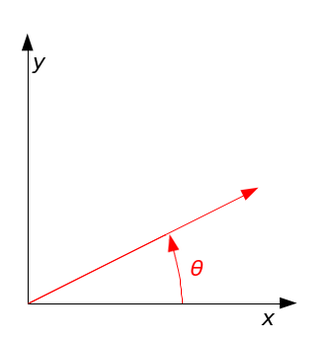
\includegraphics[width=\linewidth]{rys/givens_rot.png}
\caption{Rotacja Givensa \citep{ilustracja}}\label{rys:logo:jeden}
\end{figure}

\begin{definition}[Macierz Givensa]
Niech $ i,j \in {1, \ldots, n}$ i $\theta \in \setR$. Macierz $\mx{R}(i,j,\theta) \in \setR^{n\times n}$ zdefiniowana następująco:
$$
\mx{R}(i,j,\theta) = \begin{bmatrix}
1       & 0     & \cdots &    0       & \cdots &    0       & \cdots & 0 & 0& \\
0       & 1     & \cdots &     0      & \cdots &     0      &  \cdots& 0 & 0 &   \\
0       & 0     & \ddots &     0      &  \cdots&     0      &  \cdots& 0 & 0 &  \\
\vdots  &\vdots &  \cdots& \cos\theta & \cdots & -\sin\theta&  \cdots& 0 & 0& \\
0       &  0    & \cdots & \vdots     &  \ddots&  \vdots    & \cdots & 0 & 0& \\
\vdots  & \vdots& \cdots & \sin\theta & \cdots & \cos\theta &  \cdots& 0 & 0& \\
0       & 0     & \cdots &    0       &  \cdots&  0         & \ddots &  0& 0& \\
\vdots  & \vdots&\cdots  &  \cdots    &  \cdots&  \cdots    & \cdots & 1 & 0&\\
0       & 0     & \cdots &     0      &  \cdots&    0       &  \cdots& 0 & 1 & \\       
\end{bmatrix}
$$
nazywamy macierzą rotacji Givensa.
\end{definition}

\begin{lemma}[O macierzy Givensa]
Każda macierz Givensa jest macierzą ortogonalną.
\end{lemma}

\begin{proof}
Niech $n\in \setN$, rozważmy macierze Givensa rozmiaru $n$ na $n$. Niech $i,j \in \{1,\ldots, n\}$ i $\theta \in \setR$. Pokażemy, że macierz $\mx{R}(i,j,\theta) \in \setR^{n\times n}$ jest ortogonalna.
Wystarczy pokazać, że układ kolumn $(r_s)$, $s=1,\ldots, n$ tej macierzy jest układem ortonormalnym. Weźmy dwie kolumny $k$-tą i $l$-tą. Rozważmy przypadki:
\begin{enumerate}
\item Gdy $k\notin (i,j)$, $l\notin (i,j)$, $k \neq l$, wtedy
$$
(\vr{r}_{k}|\vr{r}_{l}) = ([0,\ldots, 0,1,0,\ldots,0]|[0,\ldots,0,0,1,0,\ldots,0]) = 0
$$
$$
(\vr{r}_{k}|\vr{r}_{k}) = ([0,\ldots, 0,1,0,\ldots,0]|[0,\ldots,0,1,0,\ldots,0]) = 1
$$
\end{enumerate}

2.$k \in (i,j)$, $l \in (i,j)$, $k \neq l$
{\scriptsize
$$
(\vr{r}_{i}|\vr{r}_{j}) = ([0,\ldots, 0,\cos\theta,0,\ldots,0,\sin\theta,0,\ldots,0]|[0,\ldots, 0,-(\sin\theta),0,\ldots,0,\cos\theta,0,\ldots,0]) = \cos\theta\cdot(-\sin\theta) + \sin\theta\cdot\cos\theta = 0
$$
$$
(\vr{r}_{i}|\vr{r}_{i}) = ([0,\ldots, 0,\cos\theta,0,\ldots,0,\sin\theta,0,\ldots,0]|[0,\ldots, 0,\cos\theta,0,\ldots,0,\sin\theta,0,\ldots,0]) = \cos^{2}\theta + \sin^{2}\theta = 1
$$
$$
(\vr{r}_{j}|\vr{r}_{j}) = ([0,\ldots, 0,-(\sin\theta),0,\ldots,0,\cos\theta,0,\ldots,0]|[0,\ldots, 0,-(\sin\theta),0,\ldots,0,\cos\theta,0,\ldots,0]) = -\sin^{2}\theta + \cos^{2}\theta = 1
$$
}
3. $k=j$, $l\notin (i,j)$
$$
(\vr{r}_{j}|\vr{r}_{l}) = (\vr{r}_{l}|\vr{r}_{j})= ([0,\ldots, 0,1,0,\ldots,0]|[0,\ldots, 0,-(\sin\theta),0,\ldots,0,\cos\theta,0,\ldots,0]) = 0
$$
4. $k=i$, $l\notin(i,j)$
$$
(\vr{r}_{i}|\vr{r}_{l}) = (\vr{r}_{l}|\vr{r}_{i})= ([0,\ldots, 0,1,0,\ldots,0]|[0,\ldots, 0,\cos\theta,0,\ldots,0,\sin\theta,0,\ldots,0] = 0
$$

Z uwagi na symetrię oznaczeń, również przypadek gdy $k\notin{i,j}$, $l=i \lor l=j$, to ich iloczyn skalarny jest równy $0$. Podsumowując powyższe przypadki z dowolności wyboru kolumn $k$-tej i $l$-tej układ kolumn $r(s)$ jest ortonormalny. Zatem macierz Givensa jest ortogonalna.
\end{proof}

\begin{lemma}
Niech $\mx{A} \in \setR^{n \times n}$, $i,j \in \{1, \ldots, n\}$ oraz $\sqrt{a_{ii}^{2} + a_{ji}^{2}} > 0$. Wtedy macierz Givensa $\mx{R}(i,j, \theta)$, gdzie $\theta$ spełnia warunki:
$$
\cos\theta = \frac{a_{ii}}{\sqrt{a_{ii}^{2} + a_{ji}^{2}}}
$$
$$
\sin\theta = \frac{-(a_{ji})}{\sqrt{a_{ii}^{2} + a_{ji}^{2}}}
$$
powoduje, że jeśli $[b_{ij}]_{i=1,\ldots,n}^{j=1,\ldots,n} = \mx{B} = \mx{R}(i,j,\theta)\cdot \mx{A}$, to 
$b_{ji}=0$.
\end{lemma}

\begin{proof}
Niech $\mx{A} \in \setR^{n \times n}$, $i,j \in \{1,\ldots,n\}$, $\sqrt{a_{ii}^{2} + a_{ji}^{2}} > 0$ i $\theta$ spełniająca warunki. Niech $\mx{B} = \mx{R}(i,j,\theta)\cdot \mx{A}$. Wtedy 
$$
b_{ji}= \sin\theta\cdot a_{ii} + \cos\theta\cdot a_{ji} = \frac{-(a_{ji})}{\sqrt{a_{ii}^{2} + a_{ji}^{2}}} \cdot a_{ii} + \frac{a_{ii}}{\sqrt{a_{ii}^{2} + a_{ji}^{2}}} \cdot a_{ji} = 0.
$$
\end{proof}
Zatem macierz $\mx{R}(i,j,\theta)$ można użyć do "generowania zer w macierzy".
\begin{algorithm}
\caption{Algorytm QR metodą rotacji Givensa}
\begin{algorithmic}
\For{$i$ from $1$  to $\min (m-1,n)$}
	\For{$j$ from $i+1$ to $m$}
		\State $\mx{G} = Givens(i,j, \mx{A}[i,i], \mx{A}[j,i])$
		\State $\mx{A} = \mx{G}\cdot \mx{A}$
	\EndFor	
\EndFor
\end{algorithmic}
\end{algorithm}

\begin{proposition} \label{Proposition-zachowanie-zer}
Zauważmy jak zachowuje się macierz przy mnożeniu przez macierz Givensa.
{
\begin{equation*}
\begin{array}{c}
\begin{bmatrix}
I & 0 & 0 & 0 & 0 \\
0 & \cos\theta & 0 & -\sin\theta & 0 \\
0 & 0 & I & 0 & 0 \\
0 & \sin\theta & 0 & \cos\theta & 0 \\
0 & 0 & 0 & 0 & I
\end{bmatrix} \cdot \begin{bmatrix}
A_{11} & A_{12} & A_{13} & A_{14} & A_{15} \\
A_{21} & A_{22} & A_{23} & A_{24} & A_{25} \\
A_{31} & A_{32} & A_{33} & A_{34} & A_{35} \\
A_{41} & A_{42} & A_{43} & A_{44} & A_{45} \\
A_{51} & A_{52} & A_{53} & A_{54} & A_{55}
\end{bmatrix} = \\ \\
{\scriptsize
\begin{bmatrix}
A_{11} & A_{12} & A_{13} & A_{14} & A_{15} \\
\cos\theta \cdot A_{21} - \sin\theta\cdot A_{41} & \cos\theta \cdot A_{22}- \sin\theta\cdot A_{42} & \cos\theta \cdot A_{23}- \sin\theta\cdot A_{43} & \cos\theta \cdot A_{24}- \sin\theta\cdot A_{44} & \cos\theta \cdot A_{25}- \sin\theta\cdot A_{45} \\
A_{31} & A_{32} & A_{33} & A_{34} & A_{35} \\
\sin\theta\cdot A_{21} + \cos\theta\cdot A_{41} & \sin\theta\cdot A_{22} + \cos\theta\cdot A_{42} & \sin\theta\cdot A_{23} + \cos\theta\cdot A_{43} & \sin\theta\cdot A_{24} + \cos\theta\cdot A_{44} & \sin\theta\cdot A_{25} + \cos\theta\cdot A_{45} \\
A_{51} & A_{52} & A_{53} & A_{54} & A_{55} 
\end{bmatrix}
}
\end{array}
\end{equation*}
}
\end{proposition}

\begin{proposition}\label{Proposition-zera-w-kolumnie}
Na podstawie obserwacji \ref{Proposition-zachowanie-zer} możemy wywynioskować następujące:
\begin{enumerate}
\item Wykonanie rotacji macierzą $\mx{G}(i,j, \mx{A}[i,i], \mx{A}[j,i])$ zachowuje zera w kolumnie $i$.
\item Wykonanie rotacji macierzą $\mx{G}(i,j, \mx{A}[i,i], \mx{A}[j,i])$ zachowuje zera w kolumnach $[1:i-1]$ w wierszach różnych od $i$ oraz $j$.
\end{enumerate}
\end{proposition}

\begin{proof}[Szkic dowodu]
Krótko uzasadnimy \ref{Proposition-zera-w-kolumnie}.
\begin{enumerate}
\item Istotnie z obserwacji \ref{Proposition-zachowanie-zer} po wykonaniu obrotu Givensa względem $i$ i $j$ inne zera będą reprezentowane przez pola $\mx{A}_{12}, \mx{A}_{32}, \mx{A}_{52}$ i w efekcie nie ulegają zmianie.
\item Istotnie z obserwacji \ref{Proposition-zachowanie-zer} po wykonaniu obrotu Givensa względem $i$ i $j$ w kolumnach $[1:i-1]$ w wierszach różnych od $i$ i $j$ są reprezentowane przez pola $\mx{A}_{11},\mx{A}_{31},\mx{A}_{51}$.
\end{enumerate}
\end{proof}



\begin{proposition}\label{Proposition-zera-w-wierszach}
Wykonanie rotacji macierzą $\mx{G}(i,j, \mx{A}[i,i], \mx{A}[j,i])$ zachowuje zera w wierszach $i$, $j$ na miejscach $\mx{A}[i,1:i]$, $\mx{A}[j, 1:i]$. 
\end{proposition}
\begin{proof}[Szkic dowodu]

Istotnie załóżmy, że $\mx{G}(i,j, \mx{A}[i,i], \mx{A}[j,i])$ są wypełnione zerami. Odpowiada to polom $\mx{A}_{21}$, $\mx{A}_{41}$. Wtedy po rotacji mamy 
$$
\overline{\mx{A}}_{21} = \cos\theta\mx{A}_{21} - \sin\theta\mx{A}_{41} = 0,
$$  
$$
\overline{\mx{A}}_{41} = \sin\theta\mx{A}_{21} - \cos\theta\mx{A}_{41} = 0.
$$
\end{proof}


\begin{example} Poniżej zilustrujemy etapy obliczania rozkładu $\mx{QR}$ macierzy $4$ na $4$ przy użyciu rotacji Givensa.
Dla $i=1$
$$
\begin{bmatrix}
x & x & x & x \\
x & x & x & x \\
x & x & x & x \\
x & x & x & x   
\end{bmatrix} \underrightarrow{\mx{G}(1,2)} \begin{bmatrix}
x & x & x & x \\
0 & x & x & x \\
x & x & x & x \\
x & x & x & x   
\end{bmatrix} \underrightarrow{\mx{G}(1,3)} \begin{bmatrix}
x & x & x & x \\
0 & x & x & x \\
0 & x & x & x \\
x & x & x & x   
\end{bmatrix} \underrightarrow{\mx{G}(1,4)} \begin{bmatrix}
x & x & x & x \\
0 & x & x & x \\
0 & x & x & x \\
0 & x & x & x   
\end{bmatrix}  
$$
Dla $i=2$
$$
\begin{bmatrix}
x & x & x & x \\
0 & x & x & x  \\
0 & x & x & x \\
0 & x & x & x  \\
0 & x & x & x 
\end{bmatrix}  \underrightarrow{\mx{G}(2,3)} \begin{bmatrix}
x & x & x & x \\
0 & x & x & x \\
0 & 0 & x & x \\
0 & x & x & x   
\end{bmatrix} \underrightarrow{\mx{G}(2,4)} \begin{bmatrix}
x & x & x & x \\
0 & x & x & x \\
0 & 0 & x & x \\
0 & 0 & x & x   
\end{bmatrix} 
$$   
Dla $i=3$
$$
\begin{bmatrix}
x & x & x & x \\
0 & x & x & x \\
0 & 0 & x & x \\
0 & 0 & x & x   
\end{bmatrix} \underrightarrow{\mx{G}(3,4)} \begin{bmatrix}
x & x & x & x \\
0 & x & x & x \\
0 & 0 & x & x \\
0 & 0 & 0 & x   
\end{bmatrix} 
$$
\end{example}
Na mocy obserwacji \ref{Proposition-zera-w-kolumnie} i \ref{Proposition-zera-w-wierszach} widzimy, że wykonanie obrotu Givensa zgodnie z zaprezentowanym wyżej przykładem zachowuje odpowiednie zera w macierzy.
Z książki Demmela \citep{demmel12} możemy uzyskać informację, że koszt  rozkładu $\mx{QR}$ za pomocą rotacji Givensa jest dwa razy większy niż koszt rozkładu za pomocą metody Householdera.






\chapter{Eksperymenty numeryczne}

\section{Algorytm dekompozycji QR metodą odbić Householdera}

Algorytm dekompozycji QR metodą odbić Householera posiada dwie główne składowe. Pierwszym z nich jest funkcja odnajdująca odpowiednie odbicie.  Odbicie reprezentowane jest przez wektor normalny do płaszczyzny odbicia. Zadaniem jest skonstruowanie odbicia, które umożliwia ''wyzerowanie'' elementów położonych poniżej przekątnej w macierzy. Kod odpowiadający poszukiwaniu takiego wektora prezentujemy poniżej:

\begin{Schunk}
\begin{Sinput}
> house = function(x) {
+   norm_x = sqrt(t(x) %*% x)
+   if (x[1] > 0) {
+     x[1] = x[1] + norm_x;
+   } else {
+     x[1] = x[1] - norm_x;
+   }
+   return(x)
+ }
\end{Sinput}
\end{Schunk}

Wtedy algorytm rozkładu QR może być zapisany za pomocą poniższego kodu:

\begin{Schunk}
\begin{Sinput}
> qr_householer = function(A)
+ {
+  R = A
+  dimm = dim(A)
+  n = dimm[2]
+   m = dimm[1]
+   Q = diag(n)
+   for (i in 1:min(m-1,n)){
+     u = house(R[i:m,i])
+     den =  (t(u) %*% u)[1,1]
+     P = diag(n+1-i) - 2/den * ( u%*% t(u)  ) 
+     R[i:m,i:n] = P %*% R[i:m,i:n]
+     if (i>1)
+       Q[i:n,1:(i-1)] = P %*% Q[i:n,1:(i-1)]
+     Q[i:n,i:n] = P %*% Q[i:n,i:n]
+   }
+   return(list(R=R, Q=t(Q)))
+ }
\end{Sinput}
\end{Schunk}

Algorytm rozpoczynamy od zadeklarowania wymiarów rozkładanej macierzy. Następnie iteracyjnie wyznaczamy odbicia reprezentowane przez wektory normalne, które są wykorzystywane do obliczenia macierzy $\mx{P}$, dzięki której obliczamy macierz trójkątną górną $\mx{R}$ oraz macierz $\mx{Q}$. Warto nadmienić również, że w jednej iteracji dokonujemy wyzerowania wszystkich elementów danej kolumny pod przekątną. Cały algorytm zwraca nam macierz $\mx{R}$ oraz co ważne zwraca nam transpozycję macierzy $\mx{Q}$.

\section{Algorytm dekompozycji QR metodą rotacji Givensa}

Algorytm dekompozycji QR metodą rotacji Givensa podobnie jak w metodzie odbić Householdera również posiada dwie główne składowe. Pierwszą z nich jest funkcja odnajdująca odpowiednią rotację, która reprezentowana jest przez macierz Givensa. Zadaniem jest skonstruowanie takiej macierzy rotującej, która umożliwia ''wyzerowanie'' w kolejnych kolumnach elementów położonych poniżej przekątnej w macierzy. Kod odpowiadający poszukiwaniu takiej macierzy prezentujemy poniżej:

\begin{Schunk}
\begin{Sinput}
> givens = function(i,j,A){
+   dimm = dim(A)
+   n = dimm[1]
+   G = diag(n)
+   p = sqrt((A[i,i])^2 + (A[j,i])^2)
+   G[i,i] = A[i,i]/ p
+   G[i,j] = (A[j,i])/p
+   G[j,i] = -(A[j,i])/p
+   G[j,j] = A[i,i]/ p
+   
+ return(G)  
+   
+ }
\end{Sinput}
\end{Schunk}

Teraz tworzymy algorytm dekompozycji macierzy QR metodą rotacji Givensa:

\begin{Schunk}
\begin{Sinput}
> qr_givens = function(A){
+   R = A
+   
+   n = dim(A)[2]
+   m = dim(A)[1]
+   Q = diag(n)
+   for (i in 1:(n-1)) {
+     for (j in (i+1):m) {
+       G = givens(i,j,R)
+       R = G %*% R
+       Q = Q %*% t(G)
+     }
+   }
+   return(list(R=R, Q=Q))
+ }
\end{Sinput}
\end{Schunk}

Algorytm rozpoczynamy od zadeklarowania wymiarów rozkładanej macierzy. Następnie iteracyjnie wyznaczamy macierz rotacji Givensa, dzięki której obliczamy macierz trójkątną górną $\mx{R}$ oraz macierz $\mx{Q}$. Warto nadmienić również, że w jednej iteracji tego algorytmu dokonujemy wyzerowania dokładnie jednego elementu danej kolumny pod przekątną. Stąd liczba iteracji jest znacznie większa niż w algorytmie qr householder. Cały algorytm zwraca nam macierz $\mx{R}$ oraz w przeciwieństwie do algorytmu qr householder zwraca nam macierz $\mx{Q}$.


\section{Eksperymenty numeryczne - porównanie jakości dwóch algorytmów}

Teraz czas na eksperymenty, które sprawdzą, jak bardzo dokładność naszych algorytmów różni się od gotowej funkcji R, służącej do rozkładu QR.
Do wyżej wymienionych eksperymentów wykorzystamy losowo wybrane trzy macierze.
\begin{enumerate}
\item Wymiarów $5$ na $5$,
\item Wymiarów $25$ na $25$, oraz
\item Wymiarów $125$ na $125$.
\end{enumerate}


\subsection{Test dla macierzy małych rozmiarów}
Na początek zajmijmy się macierzą wymiarów 5 na 5. Zostanie ona wygenerowana z losowych liczb.

\begin{Schunk}
\begin{Sinput}
> set.seed(2019)
> M_1<-matrix(c(replicate(5, rnorm(5)) ), 5, 5, byrow=TRUE)
\end{Sinput}
\end{Schunk}

Najpierw przeprowadzimy rozkład opracowanym samodzielnie algorytmem qr givens.

\begin{Schunk}
\begin{Sinput}
> wynik1_givens = qr_givens(M_1)
\end{Sinput}
\end{Schunk}

Następnie przeprowadzimy rozkład również opracowanym samodzielnie algorytmem qr householder.

\begin{Schunk}
\begin{Sinput}
> wynik1_householder = qr_householer(M_1)
\end{Sinput}
\end{Schunk}

Pozostało przeprowadzić rozkład wbudowaną funkcją w pakiet R.

\begin{Schunk}
\begin{Sinput}
> QR = qr(M_1)
\end{Sinput}
\end{Schunk}

Należy sprawdzić, który rozkład jest najbliższy naszej wyjściowej macierzy A.

Policzymy kolejno błędy bezwględne z:
\begin{enumerate}
\item Rozkładu QR metodą rotacji Givensa.
\item Rozkładu QR metodą odbić Householdera.
\item Rozkładu QR funkcją wbudowaną w język R.
\end{enumerate}

1.

\begin{Schunk}
\begin{Sinput}
> M_1_givens = wynik1_givens$Q  %*% wynik1_givens$R
> M_11 = M_1_givens - M_1
> blad_givens_M_1 = norm(M_11)
> blad_givens_M_1
\end{Sinput}
\begin{Soutput}
[1] 2.331468e-15
\end{Soutput}
\end{Schunk}

2.

\begin{Schunk}
\begin{Sinput}
> M_1_householder = wynik1_householder$Q %*% wynik1_householder$R
> M_13 = M_1_householder - M_1
> blad_householder_M_1 = norm(M_13)
> blad_householder_M_1
\end{Sinput}
\begin{Soutput}
[1] 3.996803e-15
\end{Soutput}
\end{Schunk}

3.

\begin{Schunk}
\begin{Sinput}
> M_1_qr = qr.Q(QR) %*% qr.R(QR)
> M_12 = M_1_qr - M_1
> blad_qr_M_1 = norm(M_12)
> blad_qr_M_1
\end{Sinput}
\begin{Soutput}
[1] 1.998401e-15
\end{Soutput}
\end{Schunk}


Widzimy, że gotowy algorytm, wbudowany w R jest jednak dokładniejszy od naszych, samodzielnie napisanych. Widać również, że algorytm dekompozycji QR metodą Givensa jest lepszy od algorytmu metodą odbić Householdera. Zauważmy jednak, że nasze implementacje, nie odstają znacznie od wbudowanego w język R.

Sprawdzimy czy ta zależność znajduje zastosowania dla macierzy większych rozmiarów.

\subsection{Test dla macierzy średniego rozmiaru}

Kolej na macierz wymiarów 25 na 25.

\begin{Schunk}
\begin{Sinput}
> M_2<-matrix(c(replicate(25, rnorm(25)) ), 25, 25, byrow=TRUE)
\end{Sinput}
\end{Schunk}

Rozkład algorytmem qr givens.

\begin{Schunk}
\begin{Sinput}
> wynik2_givens = qr_givens(M_2)
\end{Sinput}
\end{Schunk}

Rozkład algorytmem qr householder.

\begin{Schunk}
\begin{Sinput}
> wynik2_householder = qr_householer(M_2)
\end{Sinput}
\end{Schunk}

Rozkład wbudowaną funkcją w Pakiet R.

\begin{Schunk}
\begin{Sinput}
> QR = qr(M_2)
\end{Sinput}
\end{Schunk}

Teraz wykonujemy dokładnie taką samą procedurę jak dla macierzy wymiarów $5$ na $5$.
Liczymy kolejno błędy bezwzględne.

1.
\begin{Schunk}
\begin{Sinput}
> M_2_givens = wynik2_givens$Q  %*% wynik2_givens$R
> M_21 = M_2_givens - M_2
> blad_givens_M_2 = norm(M_21)
> blad_givens_M_2
\end{Sinput}
\begin{Soutput}
[1] 2.93654e-14
\end{Soutput}
\end{Schunk}

2.
\begin{Schunk}
\begin{Sinput}
> M_2_householder = wynik2_householder$Q %*% wynik2_householder$R
> M_23 = M_2_householder - M_2
> blad_householder_M_2 = norm(M_23)
> blad_householder_M_2
\end{Sinput}
\begin{Soutput}
[1] 2.413347e-14
\end{Soutput}
\end{Schunk}

3.
\begin{Schunk}
\begin{Sinput}
> M_2_qr = qr.Q(QR) %*% qr.R(QR)
> M_22 = M_2_qr - M_2
> blad_qr_M_2 = norm(M_22)
> blad_qr_M_2
\end{Sinput}
\begin{Soutput}
[1] 8.574738e-15
\end{Soutput}
\end{Schunk}


Tutaj obserwujemy, że błąd bezwzględny rozkładu wbudowaną funkcją w R jest wciąż najmniejszy, natomiast w tym przypadku rozkład algorytmem qr householder jest dokładniejszy od algorytmu qr givens, czyli zależność z testu dla macierzy małych rozmiarów jest odwrócona.

\subsection{Test dla macierzy dużych rozmiarów}

Sprawdzimy dokładność algorytmów dla macierzy rozmiarów $125$ na $125$. Zbadamy również czy przy wzroście wymiarów macierzy wzrastają również poszczególne błędy. 

Wygenerujmy więc macierz:

\begin{Schunk}
\begin{Sinput}
> M_3<-matrix(c(replicate(125, rnorm(125)) ), 125, 125, byrow=TRUE) 
\end{Sinput}
\end{Schunk}

Zgodnie z procedurą jaką stosowaliśmy dla macierzy mniejszych rozmiarów, przeprowadźmy kolejno:


Rozkład algorytmem qr givens:

\begin{Schunk}
\begin{Sinput}
> wynik3_givens = qr_givens(M_3)
\end{Sinput}
\end{Schunk}

Rozkład algorytmem qr householder:

\begin{Schunk}
\begin{Sinput}
> wynik3_householder = qr_householer(M_3)
\end{Sinput}
\end{Schunk}

Rozkład funkcją qr:

\begin{Schunk}
\begin{Sinput}
> QR = qr(M_3)
\end{Sinput}
\end{Schunk}

Dalej policzymy błędy bezwględne.

1.
\begin{Schunk}
\begin{Sinput}
> M_3_givens = wynik3_givens$Q  %*% wynik3_givens$R
> M_31 = M_3_givens - M_3
> blad_givens_M_3 = norm(M_31)
> blad_givens_M_3
\end{Sinput}
\begin{Soutput}
[1] 2.709751e-13
\end{Soutput}
\end{Schunk}


2.
\begin{Schunk}
\begin{Sinput}
> M_3_householder = wynik3_householder$Q %*% wynik3_householder$R
> M_33 = M_3_householder - M_3
> blad_householder_M_3 = norm(M_33)
> blad_householder_M_3
\end{Sinput}
\begin{Soutput}
[1] 4.039776e-13
\end{Soutput}
\end{Schunk}

3.
\begin{Schunk}
\begin{Sinput}
> M_3_qr = qr.Q(QR) %*% qr.R(QR)
> M_32 = M_3_qr - M_3
> blad_qr_M_3 = norm(M_32)
> blad_qr_M_3
\end{Sinput}
\begin{Soutput}
[1] 8.038709e-14
\end{Soutput}
\end{Schunk}

\subsection{Podsumowanie}

W tym momencie możemy wysnuć wniosek, że rozmiar macierzy nie wpływa istotnie na jakość naszych samodzielnie opisanych funkcji w stosunku do gotowej funkcji w R. Są one mniej dokładne niż wbudowany, gotowy algorytm dekompozycji QR w R. Ponadto algorytm metodą rotacji Givensa nie zawsze jest jakościowo lepszy od algorytmu metodą odbić Householdera. Zależy to od wymiarów oraz od losowości rozkładanej macierzy.

Zbadamy teraz jak zachowują się błędy w poszczególnych algorytmach przy zwiększaniu wymiaru. Interesuje nas czy te błędy rosną wraz ze wzrostem wymiaru, czy też wręcz przeciwnie. 

W tym celu stworzymy wykres prezentujący jak zachowują się błędy bezwzględne trzech przedstawionych przez nas algorytmów dla macierzy wymiarów omówionych przez nas.

\begin{Schunk}
\begin{Sinput}
> wymiary<-c(5,25,125)
> bledy1<-c(blad_qr_M_1,blad_qr_M_2,blad_qr_M_3)
> bledy2<-c(blad_givens_M_1,blad_givens_M_2,blad_givens_M_3)
> bledy3<-c(blad_householder_M_1,blad_householder_M_2,blad_householder_M_3)
\end{Sinput}
\end{Schunk}

\begin{Schunk}
\begin{Sinput}
> plot(wymiary, bledy1, type = 'l', col = 'blue', ylim=c(0,5e-13), ylab = "Bledy")
> lines(wymiary, bledy2, col='green')
> lines(wymiary, bledy3, col='red')
> legend(10,4e-13, c("qr in R", "qr givens", "qr householder"), 
+        fill=c("blue", "green", "red"))
\end{Sinput}
\end{Schunk}
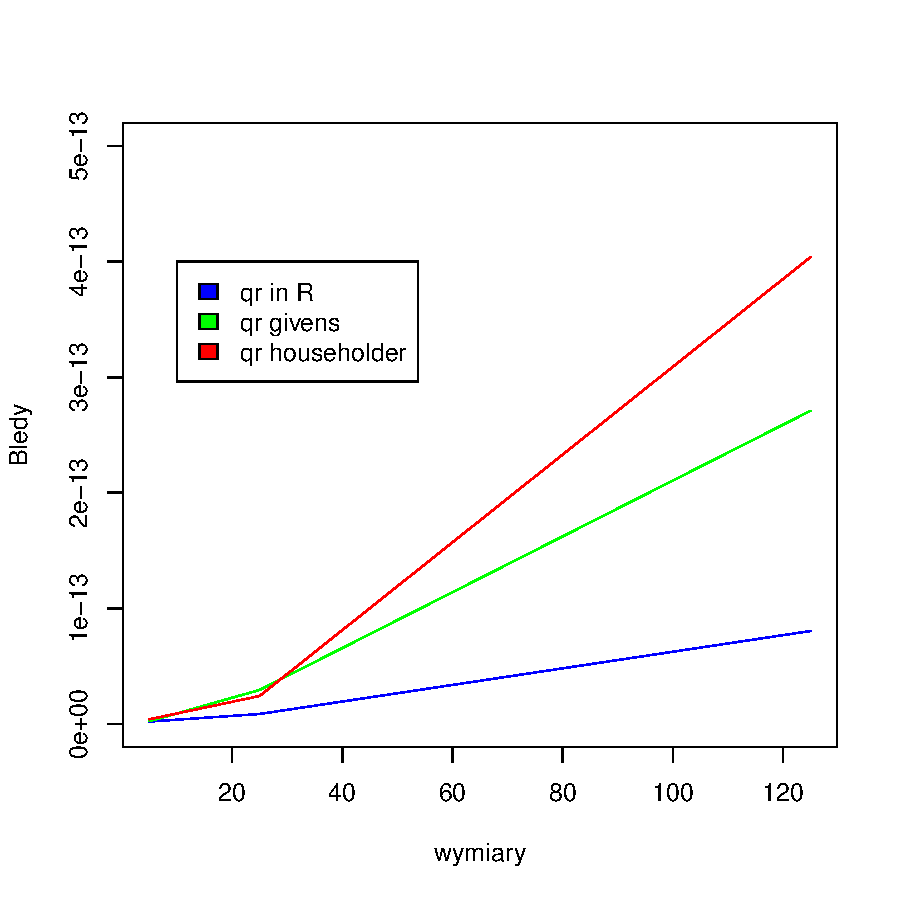
\includegraphics{licencjat-027}

Wyniki nie są zaskakujące. Wraz ze wzrostem wymiaru rosną również błędy bezwględne wszystkich przedstawionych przez nas algorytmów. Z wykresu można również zaobserwować, iż ten wzrost jest więcej niż liniowy. Warto również nadmienić, że błąd algorytmu $\mx{QR}$ metodą odbić Householdera rośnie najszybciej, zaś tempo wzrostu błędu wbudowanej funkcji jest najniższe. 



\chapter{Podsumowanie}

W pracy tej zajmowaliśmy się tematyką dotyczącą algorytmu $\mx{QR}$. W rozdziale 3 udało się zaprezentować uzupełniony dowód istnienia rozkładu $\mx{QR}$ dowolnej macierzy. Zaprezentowany dowód opiera się w głównej mierze o twierdzenie o ortogonalizacji Grama-Schmidta, przy wykorzystaniu kilku podstawowych faktów, dotyczących macierzy trójkątnych górnych i ortogonanych. Dalej w sekcjach 3.1 oraz 3.2 prezentujemy i omawiamy stabilnie numerycznie algorytmy znajdowania dekompozycji $\mx{QR}$. W seksji 3.1 algorytm $\mx{QR}$ metodą odbić Householdera, dla którego pokazujemy kilka faktów dotyczących własności macierzy odbić oraz uzasadniamy dlaczego w metodzie tej zachowane są  zera w macierzy w czasie procesu iterowania. W sekcji 3.2 prezentujemy algorytm $\mx{QR}$ metodą rotacji Givensa, wykorzystujący macierze rotacji. Również w tym wypadku dowodzimy prostych faktów dla tychże macierzy, a za pomocą obserwacji \ref{Proposition-zachowanie-zer}, \ref{Proposition-zera-w-kolumnie}, \ref{Proposition-zera-w-wierszach}  przedstawiamy czytelnikowi szkic argumentacji o zachowaniu zer w macierzy w procesie iterowania. W rozdziale 4 pracy zaprezentowaliśmy własne implementacje algorytmów, omówionych w rozdziale 3. W sekcji 4.1 znajduje się implementacja algorytmu $\mx{QR}$ metodą odbić z wykorzystaniem składni języka R. Czytenilnik znajdzie natomiast w sekcji 4.2 implementacje drugiego z algorytmów, algorytmu $\mx{QR}$ metodą rotacji. Wreszcie w sekcji 4.3 przeprowadzamy kilka prostych eksperymentów z wykorzystaniem naszych implementacji. Przeprowadzamy testy dla macierzy o rozmiarach:
\begin{enumerate}
\item 5 na 5
\item 25 na 25
\item 125 na 125
\end{enumerate}

porównując je ze sobą oraz z wbudowaną implementacją w języku R.


W efekcie przeprowadzonych eksperymentów stwierdzamy, że nasze własne implementacje niestety ustępują wbudowanej funkcji. Godnym odnotowaniem jest jednak fakt, iż uzyskane przez nie wyniki są jakościowo bliskie narzędziu wbudowanemu. Stosowanie naszych algorytmów nie powoduje bowiem wprowadzenia niedokładności większych niż $10^{-13}$ dla macierzy o rozmiarach nawet 125 na 125.




\bibliographystyle{plain}
\bibliography{bibliografia}

\end{document}
